\documentclass[11pt, a4paper]{article}

\usepackage[T1]{fontenc}
\usepackage[utf8]{inputenc}
\usepackage[polish]{babel}
\usepackage{listings}
\usepackage{mathtools}
\usepackage{blindtext}
\usepackage{scrextend}
\usepackage{graphicx}
\usepackage{amsmath}


\graphicspath{ {./images/} }


\begin{document}

\title{MOwNiT\\Laboratorium 4}
\author{Kacper Janda}
\maketitle

\section{Porównanie algorytmów rozwiązywania równań liniowych}

\begin{center}
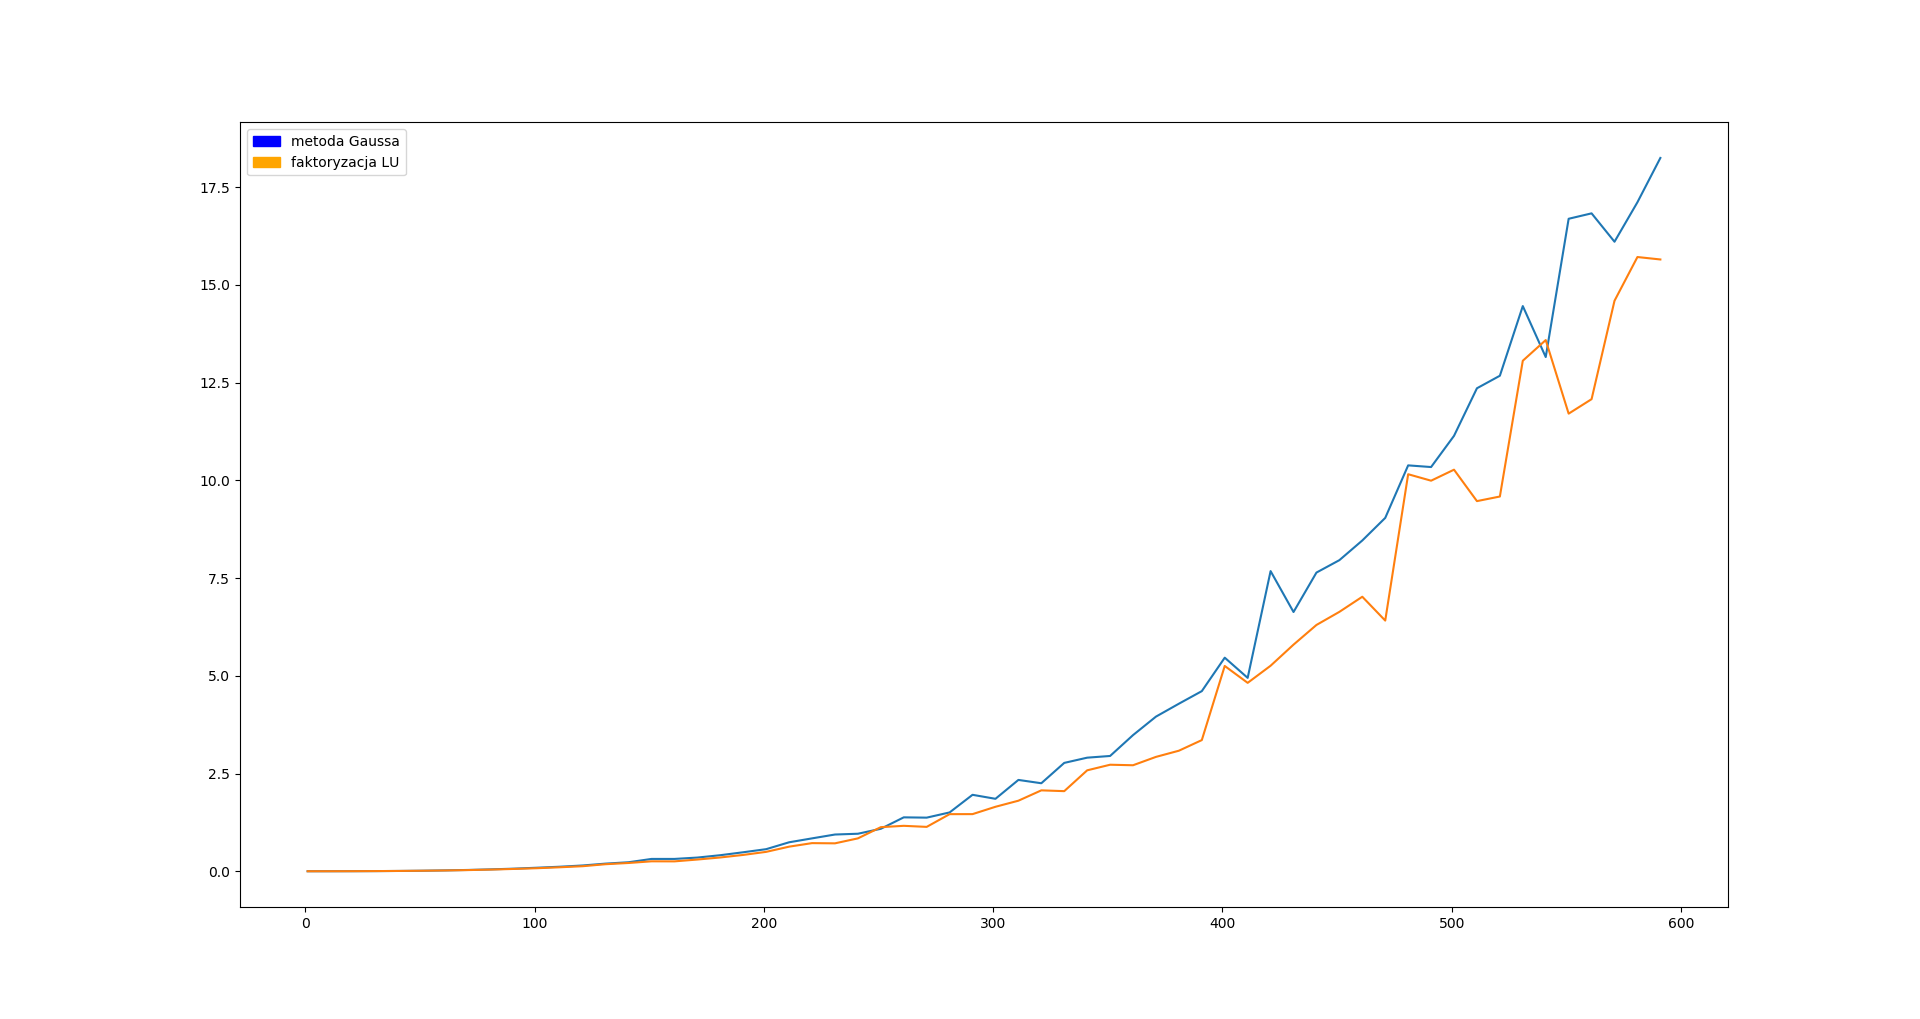
\includegraphics[scale=0.3]{Figure_2}
\end{center}

Zgodnie z przewidywaniami algorytm korzystający z faktoryzacji LU jest nieco lepszy niż klasyczna metoda Gaussa. Rząd złożoności się jednak nie zmienił - w obu metodach wynosi on \begin{math} O(n^3) \end{math}. 


\section{Porównanie algorytmów faktoryzacji LU}

\begin{enumerate}

\item Metoda Doolittle'a\\
Po rozkładzie diagonala macierzy L składa się z samych jedynek. Metoda ta zawodzi gdy diagonala macierzy A zawiera \begin{math} 0 \end{math}, ponieważ następuje wtedy dzielenie przez \begin{math} 0 \end{math}.

\item Metoda Croute'a\\
Metoda ta jest analogiczna do metody Doolittle'a za wyjątkiem tego, że w tym przypadku to macierz U zawiera same jednynki na diagonali.

\item Metoda Choleskiego
Rozkłada macierz A na macierze trójkątne L oraz U, takie że odpowiadające elementy na ich diagonalach są sobie równe. W przeciwieństwie do pozostałych metod ta pozwala obliczyć rozkład jedynie macierzy, które są symetryczne oraz dodatnio określone. Jest to spowodowane wykorzystaniem operacji pierwiastkowania w celu obliczenia wartości. Dużą zaletą tego algorytmu jest to, że po rozkładzie macierz L jest transponowaną macierzą U (\begin{math} L = U^T \end{math}).

\end{enumerate}


\end{document}